\chapter{Progettazione concettuale}
    \section{Class Diagram}

    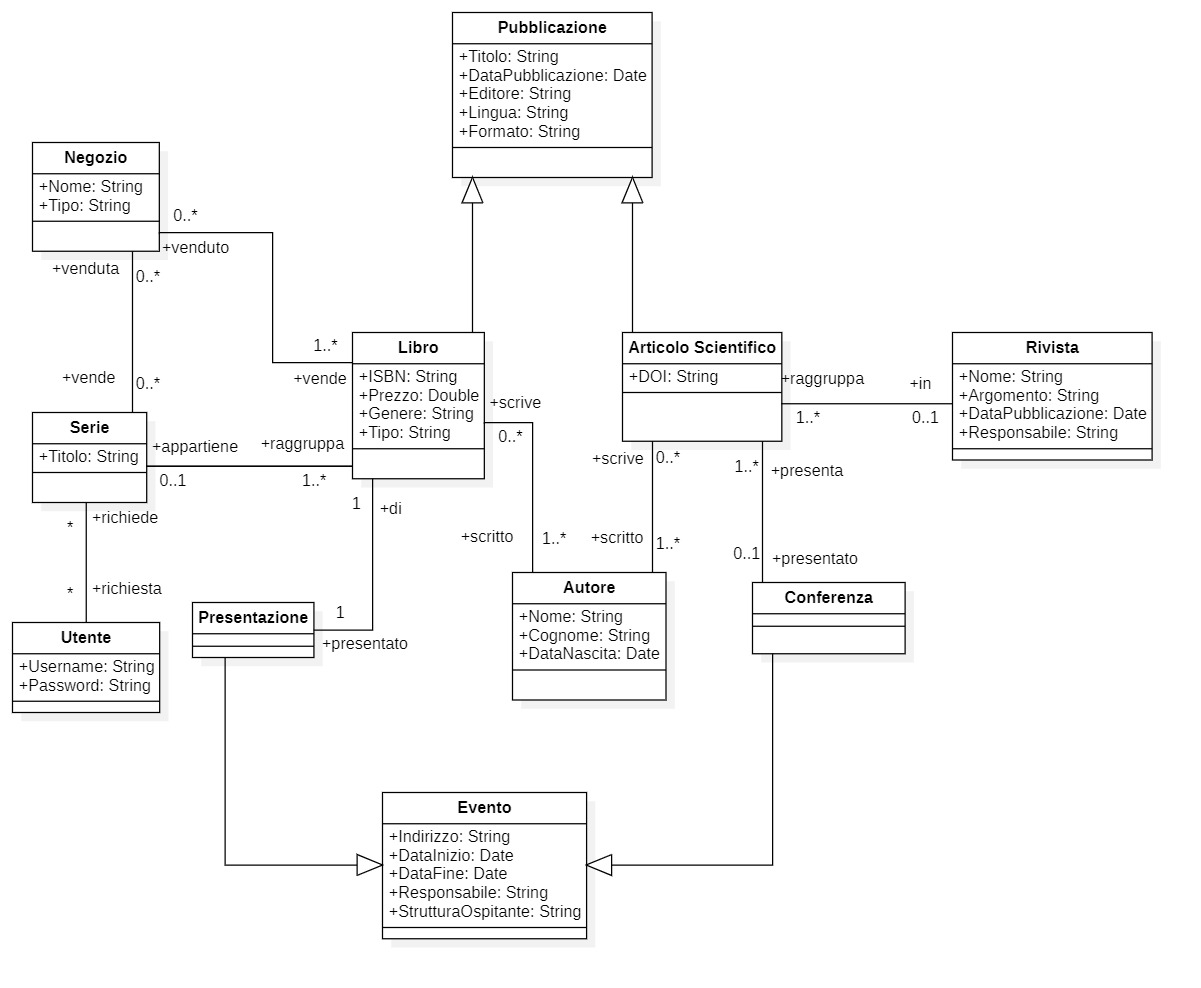
\includegraphics[scale=0.3]{Immagini/SchemaConcettuale_v1_2.png}
        
    \section{Analisi della ristrutturazione del Class Diagram}
        In questa fase verranno effettuate delle modifiche che renderanno il Class Diagram
        più adatto a una traduzione al modello logico \textcolor{red}{(magari scriviamo meglio sta parte)}
        \subsection{Analisi delle ridondanze}
        Nel Diagramma Concettuale non ci sono ridondanze tali da essere eliminate.
        \subsection{Analisi degli identificativi}
        In questa fase andremo a scegliere uno o più attributi atti a identificare univocamente
        le varie entità presenti nello schema precedente, in particolare:
            \begin{enumerate}
            \item L'entità \textbf{Libro} presenta l'attributo ISBN che rappresenta una possibile chiave primaria,
                  tuttavia è stato scelto di aggiungere un attributo \textit{ID\_Libro} in modo tale da aumentare
                  la velocità di accesso agli indici.
            \item Per \textbf{Articolo scientifico} la situazione è analoga, è stato quindi aggiunto un attributo
                  \textit{ID\_Articolo}.
            \item Nel caso dell'entità \textbf{Rivista}, la quale presenta un attributo ISSN che è chiave candidata,
                  di inserire un ulteriore attributo \textit{ID\_Rivista}.
            \item Sarebbe possibile identificare un \textbf{Evento} tramite un insieme piuttosto ampio di attributi, è
                  stato quindi aggiunto un attributo \textit{ID\_Evento}.
            \item Dato che diversi \textbf{Autori} potrebbero avere lo stesso nome, è stato aggiunto l'identificativo
                  \textit{ID\_Autore}.
            \item Dato che l'entità \textbf{Negozio} non presenta alcuna chiave candidata, è stato aggiunto l'attributo
                  \textit{ID\_Negozio}.
            \item \'E stato deciso di aggiungere a \textbf{Serie} un attributo \textit{ID\_Serie} per ridurre il volume degli
                  indici associati.
            \end{enumerate}
        \subsection{Rimozione degli attributi multivalore}
            Non sono presenti attributi multivalore.
        \subsection{Rimozione degli attributi composti}
            Non sono presenti attributi composti.
        \subsection{Partizione/Accorpamento delle associazioni}
            
        \subsection{Rimozione delle gerarchie}
            In questo diagramma sono presenti 2 generalizzazioni e 4 relative specializzazioni.
            In particolare:

            Per quanto riguarda la generalizzazione \textbf{Pubblicazione}, si è scelto di accorpare l'entità padre
            nelle entità figlie, ottenendo come risultato:
            \begin{itemize}
                  \item Una entità \textbf{Libro} aventi tutti gli attributi di \textbf{Pubblicazione} più
                        gli attributi della precedente entità \textbf{Libro}.
                  \item Analogamente, l'entità \textbf{Articolo} avrà come attributi, quelli di \textbf{Pubblicazione}
                        uniti agli attributi di \textbf{Articolo}.
            \end{itemize}
    
    \section{Class Diagram ristrutturato}
    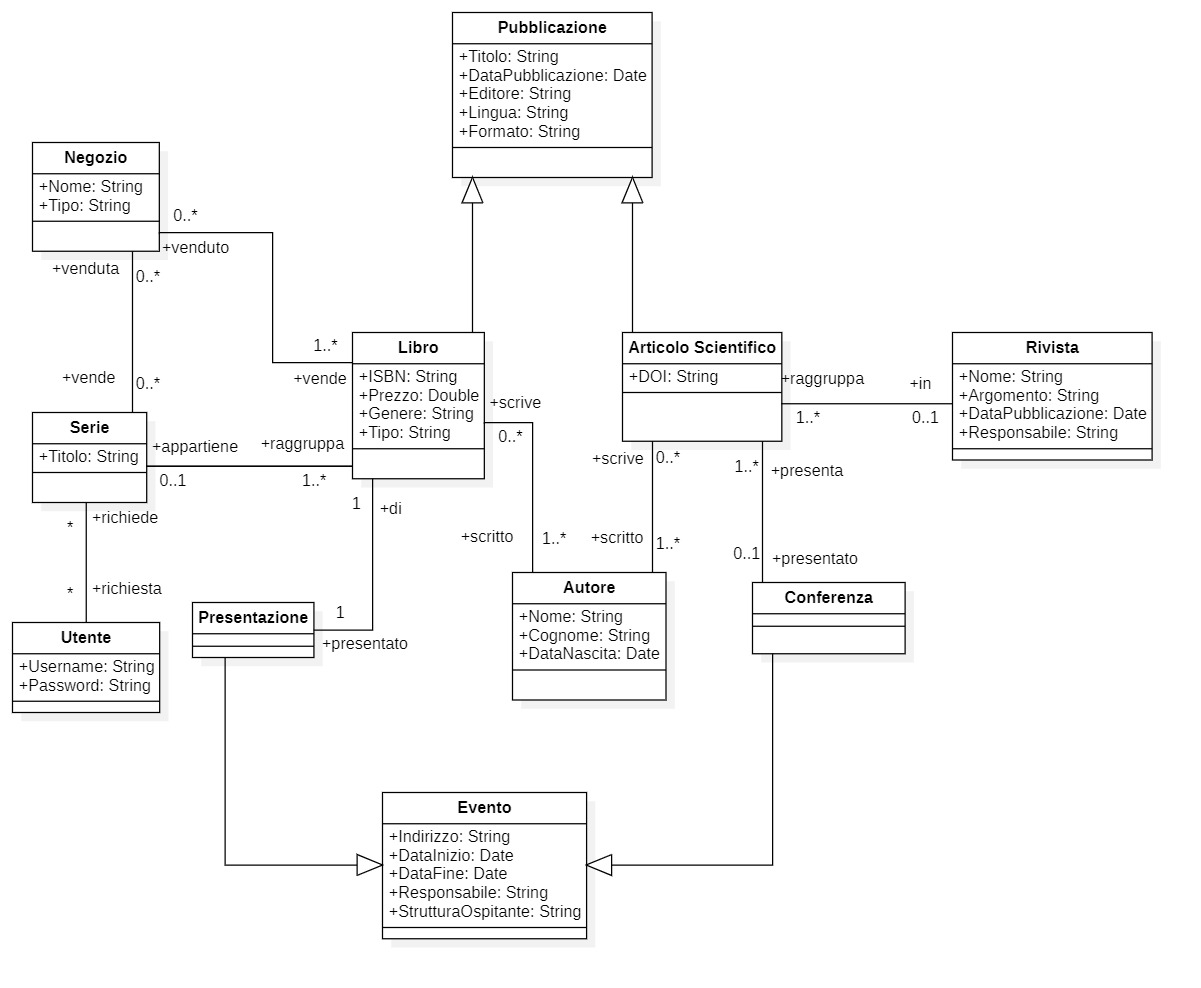
\includegraphics[scale=0.25]{Immagini/SchemaConcettuale_v1_2}
        
    \section{Dizionario delle classi}
        
    \section{Dizionario delle associazioni}